\chapter{Aspekte der Datensicherheit}
John McCumber erstellte ein Würfelmodell, welches drei Dimensionen der Datensicherheit darstellt (Cybersecurity Cube, McCumber Cube).

\begin{figure}[H]
	\centering
	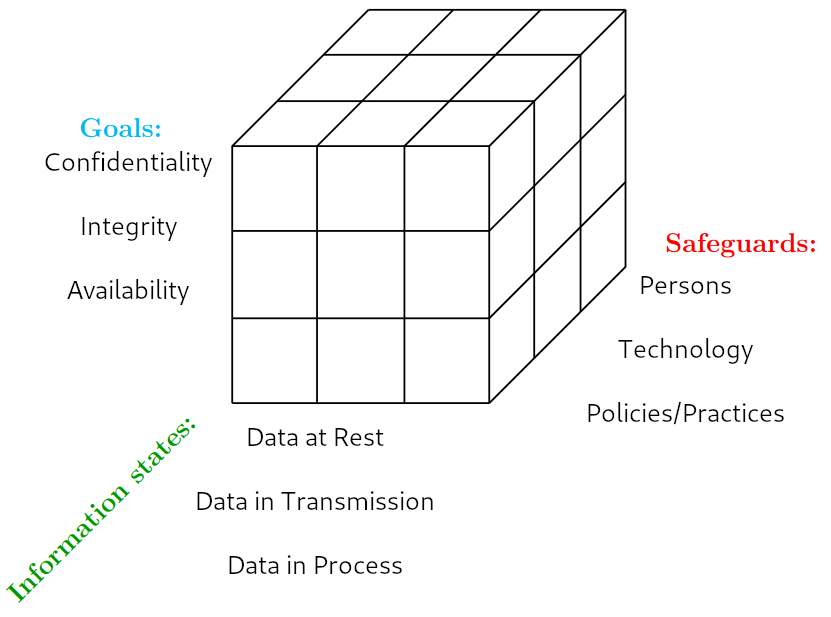
\includegraphics[width=1.0\linewidth]{figures/mccumbercube.png}
	\caption{John McCumber Cybersecurity Cube}
\end{figure}

Die dreidimensionale Darstellung des Würfels zeigt, dass die Faktoren zusammenhängen. Dementsprechend müssen alle Faktoren und ihre Verbindungen untereinander berücksichtigt werden. Der Würfel soll zu einer methodischen Vorgehensweise verhelfen.
\begin{itemize}
	\item Es ist nicht ausreichend, wenn Daten auf der Festplatte verschlüsselt abgespeichert sind, diese aber unverschlüsselt über das Internet versendet werden
	\item Ohne Policy mit Richtlinien für regelmäßige Sicherungen wird die Verfügbarkeit kaum gewährleistet, auch wenn Personen gut geschult sind und Technologie (Firewall) von Angriffen schützt (z.B. Feuer)
\end{itemize}

\begin{itemize}
	\item \textbf{Safeguards (Schutzmaßnahmen)}
	\begin{itemize}
		\item \textbf{Persons:} Bewusstseinsschulung zum Umgang mit Daten und Geräten, Erkennung von Social Engineering,...
		\item \textbf{Policies:} Definition von (in-)akzeptablen Verhalten und Ablauf bei einem Vorfall. Passwortrichtlinien, wer darf wohin, Konsequenzen definieren,...
		\item \textbf{Technology:} Software \& Hardware: Firewall, IDS, physische Zugangskontrollen,...
	\end{itemize}
	\item \textbf{Information States (Zustände)}
	\begin{itemize}
		\item \textbf{Data at Rest:} gespeicherte Daten auf HDD, SSD, USB-Stick, RAID, NAS, Cloud,...
		\item \textbf{Data In Process:} Dateneingabe, -ausgabe und -veränderung; Datenformat, Eingabefehler $\rightarrow$ Schutz gegen z.B. SQL-Injections
		\item \textbf{Data in Transmission:} Datenversendung über LAN, WLAN, Sneakernet (physischer Transport von Datenträgern mittels PKW)
	\end{itemize}
	\item \textbf{Goals (Ziele)}
	\begin{itemize}
		\item \textbf{Confidentiality (Vertraulichkeit):} Zugriffskontrolle, Verschlüsselung, Datensparsamkeit, Anonymisierung, Tokenization, Steganographie,...
		\item \textbf{Integrity (Integrität):} Konsistenzchecks, Prüfsummen
		\item \textbf{Availability (Verfügbarkeit):} häufige Probleme: DoS-Angriffe, Stromausfall. Naturkatastrophen; Sicherstellung durch Back-Ups, Redundanz, Abwehrmaßnahmen, Wartung/Reinigung von Hardware, Wiederherstellungspläne, Tests,...
	\end{itemize}
\end{itemize}

Weitere Ziele
\begin{itemize}
	\item \textbf{Authenticity (Authentizität):} Nachricht kommt vom tatsächlich behaupteten Sender
	\item \textbf{Non-repudiation (Nichtabstreitbarkeit):} Handlungen lassen sicht nicht Abstreiten z.B. durch digitale Unterschrift
	\item \textbf{Accountability (Zurechenbarkeit):} Handlung einer bestimmten Person zuordnen/zurechnen
	\item \textbf{Anonymity (Anonymität):} Aktivisten, Journalisten, Whistleblower,...
\end{itemize}







